\documentclass{article}
\usepackage[utf8]{inputenc}
\usepackage{graphicx}
\usepackage{pgfgantt}
\usepackage{lscape}
\usepackage{rotating}
\renewcommand{\refname}{Kaynakça}
\usepackage{pdflscape}
\usepackage{hyperref}
\usepackage{caption}
\usepackage{pdflscape}
\usepackage{fancyhdr}

\DeclareCaptionLabelFormat{custom}{\textbf{Figür #2}}
\captionsetup[figure]{labelformat=custom,labelsep=period}

\begin{document}

\begin{titlepage}
    \centering
    %\vspace*{0.5cm}
    
\includegraphics[width=0.3\textwidth]{ksbu.png} 
    \vskip 1em
    \vspace{1cm}
    {\scshape\Large ML-Agents Final Raporu Rapor \par}
    \vspace{1cm}
    {Yazar: Mert Koca \par}
    {\today\par}
    %\vfill
    \begin{center}
        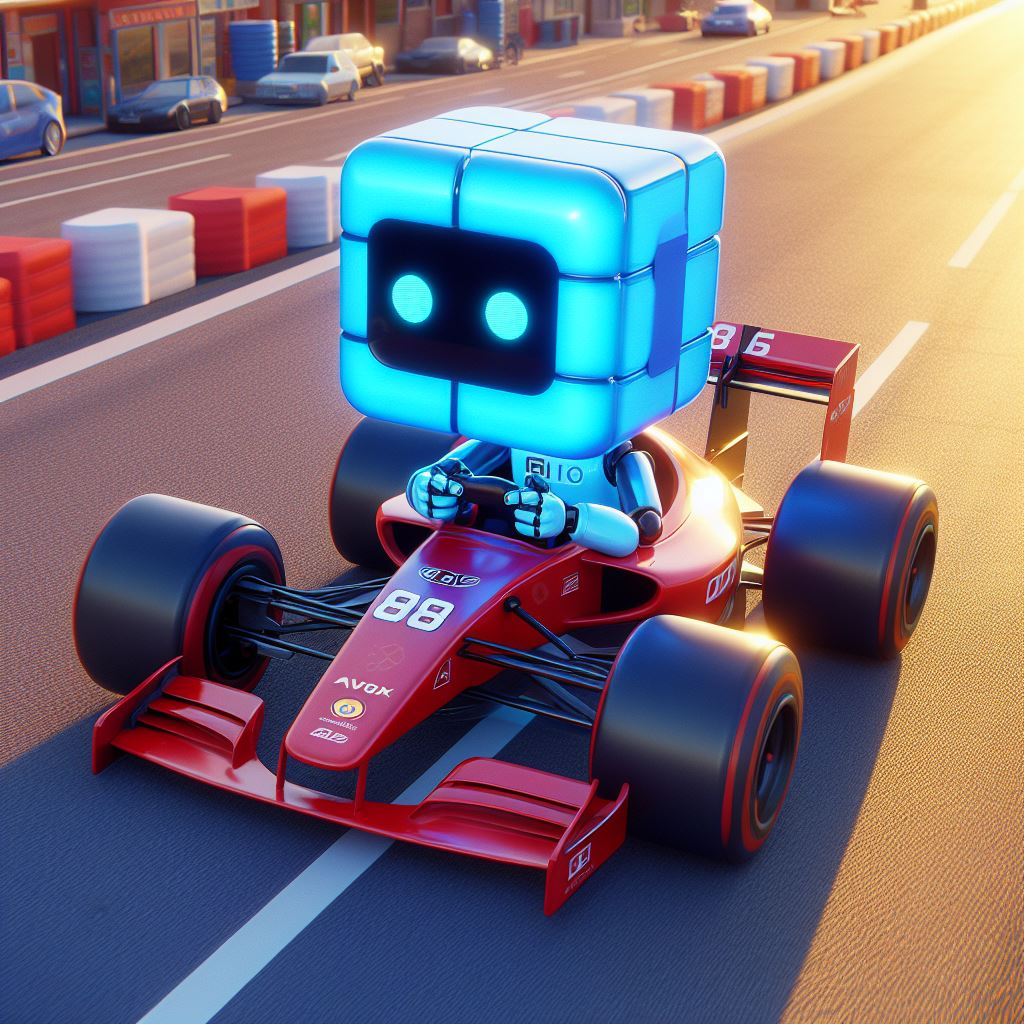
\includegraphics[width=0.5\textwidth]{gorsel.jpeg} 
    \end{center}
    \vspace{0.5cm}
    {Özet \par}
    \vspace{0.1cm}
    {Bu proje, Unity'nin ML-Agents kütüphanesi kullanılarak Python ve PyTorch ile geliştirilen bir yapay zeka projesidir. Bu proje, Unity ortamında eğitilmiş bir yapay zeka modeli oluşturarak araba sürmeyi öğretmeyi amaçlamaktadır.\par}
    \vspace{1cm}
\end{titlepage}

\newpage

\section{Giriş}
\rule{\textwidth}{0.5pt}
\par Bu projenin amacı, Unity ortamında eğitilmiş bir yapay zeka modeli oluşturarak araba sürmeyi öğretmektir. Bu rapor, projenin gereksinimlerini, literatür taramasını, teşvik öğrenme algoritmasını, kurulum aşamalarını, ML-Agents bileşenlerini, projenin farklı bölümlerini ve sonuçlarını detaylı bir şekilde ele almaktadır. Ayrıca, eğitim süreçleri ve elde edilen başarılar da raporda incelenmektedir. Bu çalışma, yapay zeka alanında ML-Agents gibi kütüphanelerin kullanımının ve uygulamalarının önemini vurgulamaktadır.\\[5pt]

\section{Gereksinimler}
\rule{\textwidth}{0.5pt}
\begin{enumerate}
    \item Python 3.9.13
    \item Unity
    \item PyTorch
    \item Visual Studio  
    \item ML-Agents Kütüphanesi\\[5pt]
\end{enumerate}

\section{Literatür}
\rule{\textwidth}{0.5pt}
\par \textbf{Python 3.9.13:} Genel amaçlı, yüksek seviyeli, etkileşimli bir programlama dilidir. Basit ve okunabilir sözdizimine sahiptir. Python, modüler yapısı ve geniş standart kütüphanesiyle birçok farklı alanda kullanılabilir.\\[5pt]

\textbf{PyTorch:} Python tabanlı ve açık kaynaklı makine öğrenmesi kütüphanesidir.\\[5pt]

\textbf{Unity:} Oyun ve grafik uygulamaları geliştirmek için kullanılan bir oyun motorudur.\\[5pt]

\textbf{ML-Agents Kütüphanesi:} Oyun ve simülasyonlarda ajanların eğitimi için ortamlar sağlayan açık kaynaklı bir projedir. Python API'ı kullanılarak teşvik öğrenmesi yöntemiyle ajanlar eğitilebilir. PyTorch tabanlı uygulamalar sunar. Ajanlar, NPC davranışlarını kontrol etmek ve oyun yapılarının otomatik test edilmesi gibi çeşitli amaçlar için kullanılabilir.


\section{Teşvik Öğrenme Algoritması}
\rule{\textwidth}{0.5pt}
\par Teşvik öğrenme algoritmasında, ajan çevresiyle etkileşime girer, belirli eylemler gerçekleştirir ve bu eylemlerin sonuçlarına göre ödüller veya ceza alır. Resimde gösterilen şema, ajanın çevresiyle olan etkileşimini ve bu süreçteki temel unsurları açıkça göstermektedir. Ajan, deneyimlediği ödül ve cezaları kullanarak en iyi eylem stratejilerini geliştirmeye çalışır.
\newline
\par Ibrahim Sobh Ibrahim'in yürüttüğü araştırma\cite{kiran2021deep}, Reinforcement Learning (RL) algoritmalarını kullanarak ajanların dinamik ortamlarda hızlı bir şekilde öğrenmesini ve adapte olmasını vurgulamaktadır. Derin RL'yi kullanarak, çalışma, özellikle müzakere gerektiren ve dinamik etkileşimler gerektiren senaryolarda otonom ajanların karar verme yeteneklerini artırmayı amaçlamaktadır.\\[5pt]

\begin{figure}[h]
    \begin{center}
        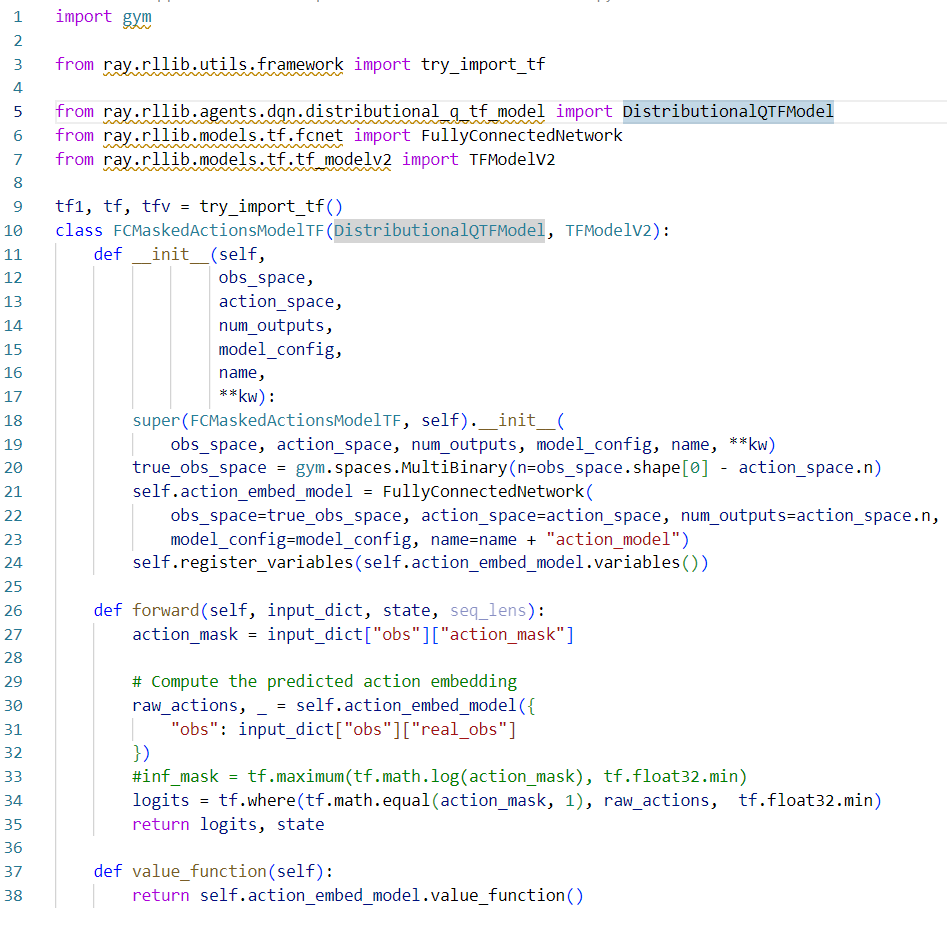
\includegraphics[width=0.7\textwidth]{model.png}
    \end{center}
      \caption{Teşvik Öğrenme Algoritması Modeli \cite{model}}
\end{figure}

\begin{enumerate}
    \item \textbf{Agent (Ajan):} Karar veren, öğrenen,  eylemleri belirleyen ve ödülü maksimize etmeye çalışan yapay zekadır.

    \item \textbf{Environment (Çevre):} Ajanın kararlarının etkileşimde bulunduğu ve ona geri bildirim sağlayan simülasyon ortamıdır.

    \item \textbf{State:} Zaman (t) anındaki çevrenin durumu ya da ajanın o andaki gözlemini temsil eder.

    \item \textbf{Action:} Ajanın zaman (t) anında yapmayı seçtiği eylemdir.

    \item \textbf{Reward:} Ajanın (t+1) anındaki eylemi sonucunda elde ettiği ödüldür

    \item \textbf{Next State:} Ajanın eylemi sonucunda çevrenin ulaştığı sonraki durumdur.
\end{enumerate}

\newpage

\section{Kurulum Aşamaları}
\rule{\textwidth}{0.5pt}
\begin{enumerate}
    \item cmd yani komut istemi çalıştırılır ve cd (dizini değiştir) komutuyla projenin olduğu dosya açılır.
    
    \item Dosyanın içinde venv adında bir virtual environment (sanal ortam) oluşturulur. Bu sayede python kullanılan başka bir proje ile karışıklık yaşanmasını önlenir.
    
    \item Oluşturulan sanal ortam aktive edilir.
    
    \item Python Package Installer (pip) güncel olup olmadığı kontrol edilir.
    
    \item ML-Agents paketi kurulur.

    \item Python torch kütüphanesi ve torch içindeki görüntü ve ses işleme kütüphanesi kurulur.
    
    \item protobuf 3.20.3 sürümü kurlur. Protobuf, veri transfer protokolü olup diğer protokollere göre daha hızlıdır.
    
    \item Packaging kütüphanesi kurulur. Bu kütüphane, python paketleri oluşturma, dağıtma ve sürümleme işlemlerini kolaylaştırır.
    
    \item Unity projesi açılıp Package Manager kısmından mlagents paketi aktif edilir.
    
    \item Boş bir nesne üretip bu nesnenin component kısmından ML-Agents aktif edilip edilmediği kontrol edilir.
    
\end{enumerate}

\newpage

\section{ML-Agents Bileşenleri}
\rule{\textwidth}{0.5pt}
\begin{enumerate}
    \item \textbf {Behavior Parameters:} Ajanların davranışlarını ve öğrenme süreçlerini kontrol etmek için kullanılan parametrelerin ayarlandığı bir bileşendir.
    \item \textbf {Buffer Sensor:} Çeşitli veri türlerini depolamak ve işlemek için kullanılan bir sensördür.
    \item \textbf {Camera Sensor:} Oyun dünyasını görsel veri olarak almak için kamera görüntülerini kullanan bir sensördür.
    \item \textbf {Decision Requester:} Ajanların kararlarını gerektiğinde talep etmelerini sağlayan bir bileşendir.
    \item \textbf {Demonstration Recorder:} Eğitim için insanların gerçekleştirdiği oyun hareketlerini kaydetmek ve kullanmak için bir kayıt cihazıdır.
    \item \textbf {Grid Sensor:} Grid tabanlı oyunlarda çevre bilgisini algılamak için kullanılan bir sensördür.
    \item \textbf {Match 3 Actuator:} Match 3 tarzı oyunlarda (Candy Crush) eylemleri gerçekleştirmek için kullanılan bir bileşendir.
    \item \textbf {Match 3 Sensor:} Match 3 tarzı oyunlarda oyun durumunu algılamak için kullanılan bir sensördür.
    \item \textbf {Ray Perception Sensor 2D/3D:} 2 boyutlu veya 3 boyutlu ortamlarda nesneleri algılamak için kullanılan bir sensördür.
    \item \textbf {Render Texture Sensor:} Görüntüleri işlemek için render texture'ları kullanarak veri sağlayan bir sensördür.
    \item \textbf {Vector Sensor:} Özel bir vektör verisiyle ajanlara çevre bilgisi sağlayan bir sensördür.\\[15pt]
\end{enumerate}

\begin{figure}
    \begin{center}
        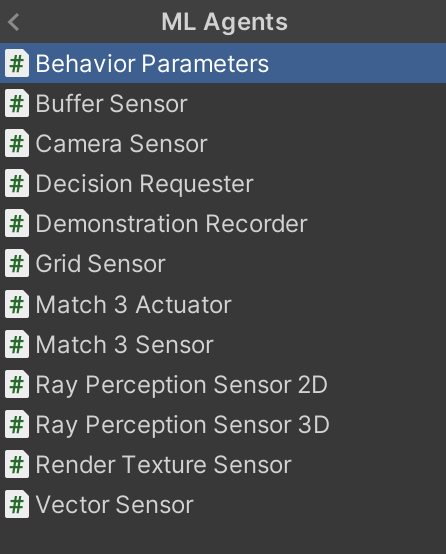
\includegraphics[width=0.9\textwidth]{mlagentcomponents.png}
    \end{center}
      \caption{ML-Agents Bileşenleri}
\end{figure}

\newpage

\section{ML-Agents Hareket Projesi}
\rule{\textwidth}{0.5pt}
Platform üzerinde mavi agentin hedeflediği mor renkli ödüller yer alır \cite{theashbot}. Bunların yanında görünmeyen ancak temas edildiğinde ceza uygulayan duvarlar da bulunmaktadır. Platformun rengi, Agent'ın etkileşimlerine göre değişmektedir. Ödül alındığında platform yeşile, duvara çarpıldığında kırmızıya dönüşür. Bu tasarım, agentin belirlenen hedeflere ulaşmasına teşvik ederken, aynı zamanda negatif etkileşimlerden kaçınma yeteneğini geliştirmeyi amaçlamaktadır. \\[5pt]

\begin{figure}[h]
    \begin{center}
        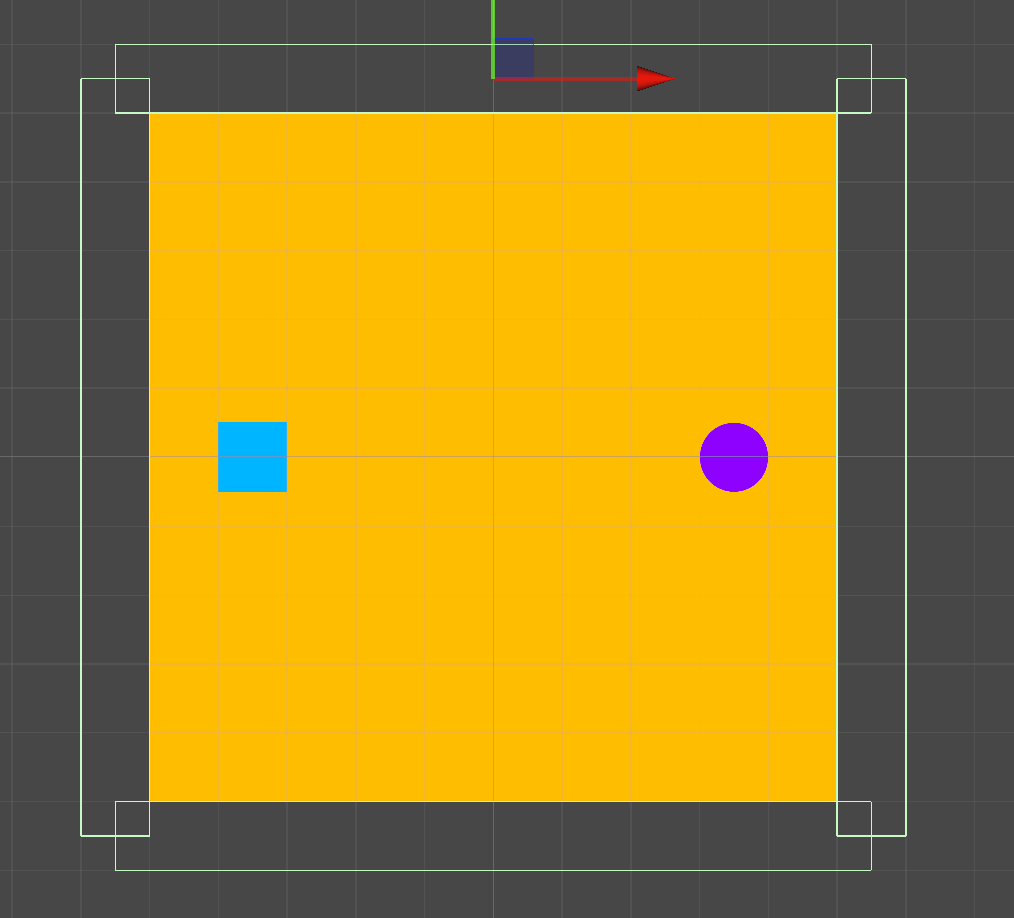
\includegraphics[width=0.8\textwidth]{duvar.png}
    \end{center}
      \caption{Hareket Projesi Bölüm Tasarımı}
\end{figure}

\newpage

\section{Proje Nesneleri}
\rule{\textwidth}{0.5pt}
Projenin bu kısmında kullanmak üzere dört adet nesne seçilmiştir. Seçilen nesneler platform, agent, ödül ve duvarlardır. Agent hareket ederek ödüle ulaşmayı hedefler fakat bu süreçte duvarlara temas ederse en baştan başlamak zorundadır.\\[5pt]

\begin{figure}[h]
    \begin{center}
        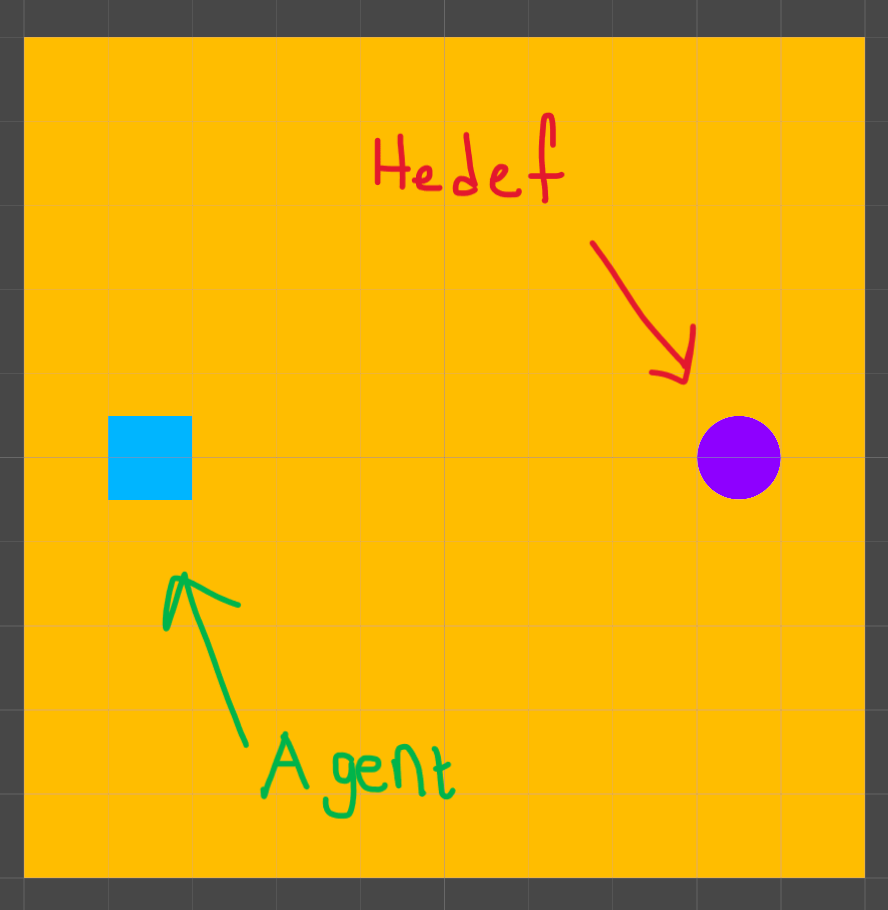
\includegraphics[width=0.9\textwidth]{agent_hedef.png}
    \end{center}
      \caption{Agent ve Hedef}
\end{figure}

\newpage

\section{ML-Agents Davranışları}
\rule{\textwidth}{0.5pt}
Agent hedefe ulaşmak için bir çok kez deneme yapmalıdır. Simulasyon hızlandırılmış olsada daha da hzılandırmak için oluşturulan bölüm koyalanarak toplamda aynı bölümden dokuz tane oluşturulmuştur. Böylece dokuz ajan aynı anda eğitilir. \\[5pt]

\begin{figure}[h]
    \begin{center}
        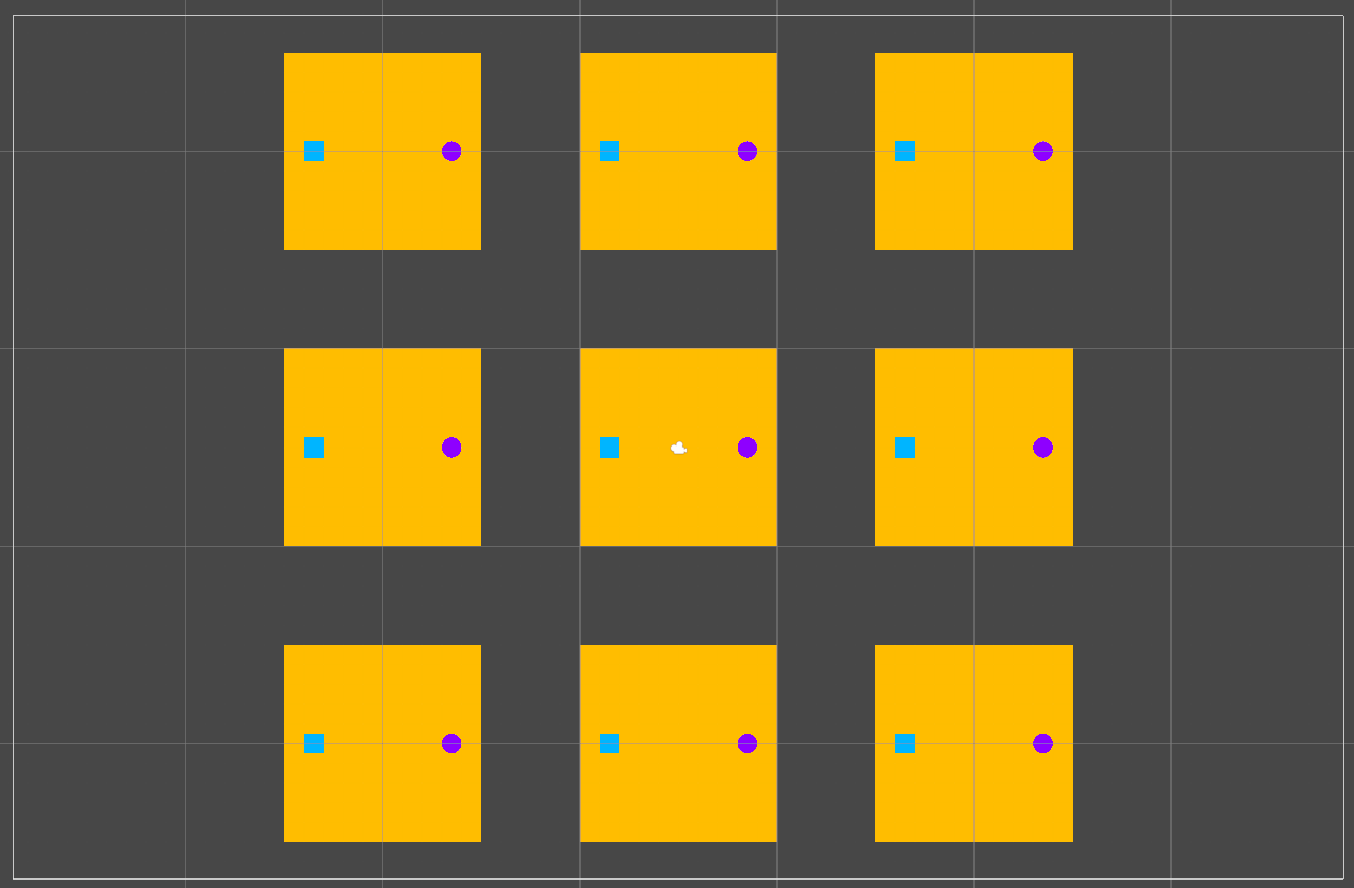
\includegraphics[width=1.1\textwidth]{coklu_bolum.png}
    \end{center}
      \caption{Çoklu Bölüm}
\end{figure}

\newpage

\section{Araç Kontrolleri Öğrenme Projesi}
\rule{\textwidth}{0.5pt}
\par Hareket Projesine benzer olarak, platform üzerinde agentin hedeflediği mor renkli ödüller yer alır. Bu ödüllerin yeri her denemede rastgele olacak şekilde değişir. Araç duvara çarparsa ceza puanı alır ve yeniden başlar, araç hedefe ulaşırsa ödül puanı alır ve yeniden başlar. Platformun rengi, Agent'ın etkileşimlerine göre değişmektedir. Ödül alındığında platform yeşile, duvara temas edildiğinde kırmızıya dönüşür. Bu tasarım, ajanların basit araç kontrollerini öğrenmesini sağlar.
\newline
\par flyyufelix adlı github kullanıcısının yaptığı "donkeyrl" projesinde\cite{flyyufelix} Donkey Car adı verilen bir arabanın bir pist etrafında RL kullanarak kendi kendine dönmesini sağlamıştır. Bu projede Double Deep Q Learning (DDQN) kullanılmıştır. DDQN, bir ajanın çevresiyle etkileşime girerek belirli bir durumda alabileceği eylemler arasında en uygun olanını seçmeyi öğrenen bir güçlendirme öğrenme algoritmasıdır.\\[15pt]

\begin{figure}[h]
    \begin{center}
        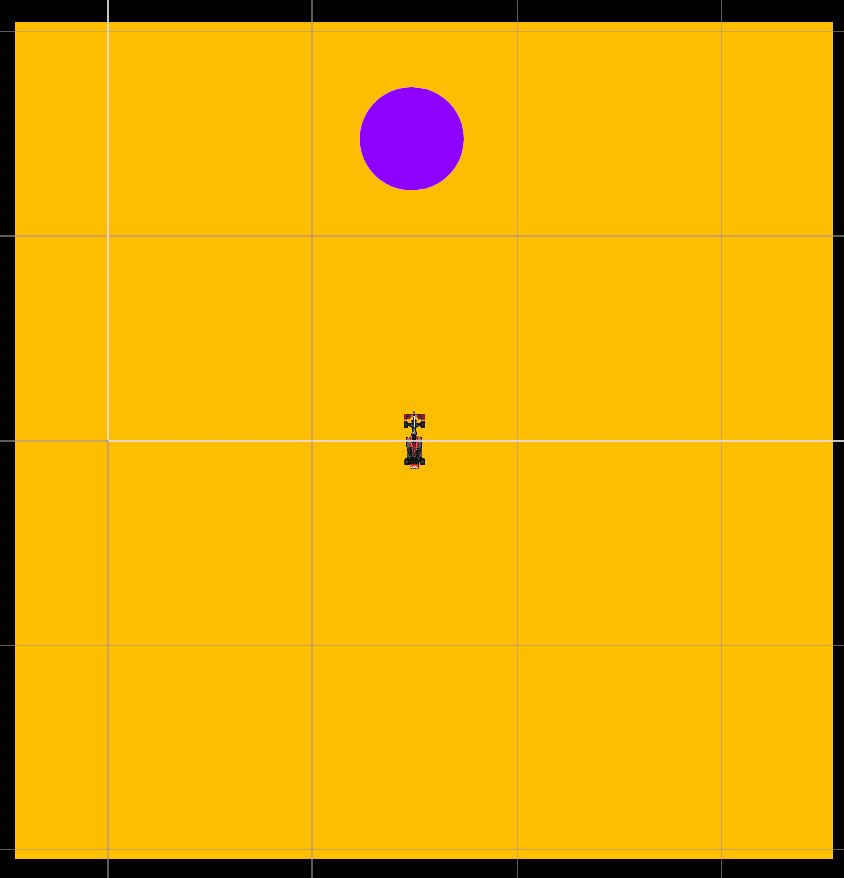
\includegraphics[width=0.7\textwidth]{tek-map.png}
    \end{center}
      \caption{Araç Kontrolleri Öğrenme Projesi Bölüm Tasarımı}
\end{figure}

\newpage

\section{Araç ve Ajan Kontrolleri}
\rule{\textwidth}{0.5pt}
\par Önceden carInput isminde başka bir koddan alınan girdiler, ajan kodunun içindeki X ekseni ve Y ekseni olarak ajan hareketlerinden alındı. Böylece ajanların araba kontrollerine erişimi sağlandı. 
\newline
\par Ajanın kullancı tarafından kontrol edilip edilemediğini, ajanın kaç eksende hareket yaptığını, eğitilen beynin ajana aktarıldığı ve diğer bir çok ayarların yapıldığı kısım Behavior Parameters olarak adlandırılır. Bu özellik ML-Agents ile birlikte gelir.\\[5pt]


\begin{figure}[h]
    \begin{center}
        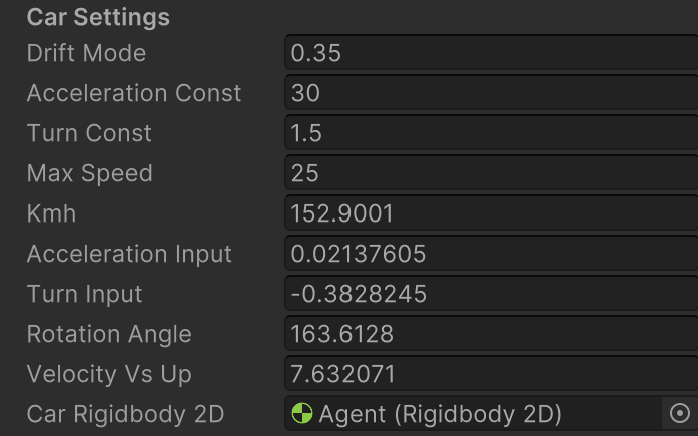
\includegraphics[width=0.65\textwidth]{kontrol.png}
    \end{center}
      \caption{Araba Kontrolleri}
\end{figure}

\begin{figure}[h]
  \centering
  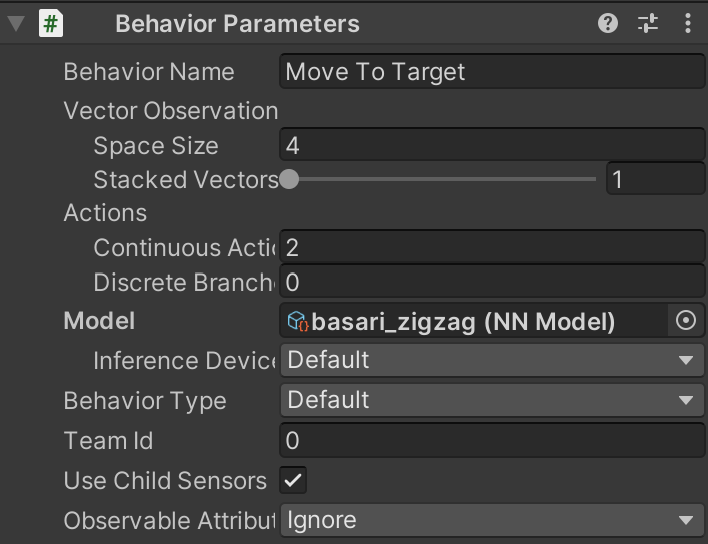
\includegraphics[width=0.65\textwidth]{behavior.png}
  \caption{Behavior Parameters}
\end{figure}

\par\textbf{Behavior Type:} Agent'ın kullancı tarafından kontrol edilip edilemediğini değiştiren bir özelliktir. Agent'ı kullanıcının  yönetmesi isteniyorsa heuristic only seçeneği seçilmelidir. Agent'a dışarıdan herhangi bir müdehalede bulunmadan hedefe ulaşması isteniliyorsa inference only seçeneği seçilmelidir.
    \newline

\begin{figure}[h]
  \centering
  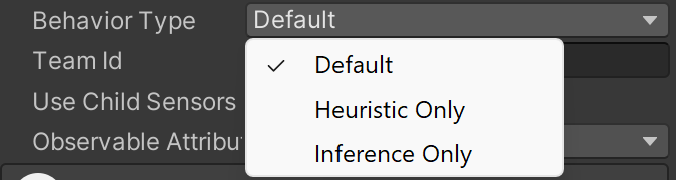
\includegraphics[width=0.9\textwidth]{behavior_type.png}
  \caption{Behavior Type}
\end{figure}

\vspace{1cm}

\par\textbf{Space Size:} Agent'ın sahip olduğu davranışları belirleyen ve yönlendiren bir özelliktir. Bazı durumlarda Agent'ın farklı davranışlar sergilemesi istenebilir. Bu durumda, her bir nesner için farklı davranışlar tanımlanması gerekir. Bu projede Agent ve Ödül olarak iki hareketli nesne olduğundan her iki nesnenin de x ve y eksenindeki hareketleri almak için Space Size özelliği dört olarak ayarlanır.
    \newline

\begin{figure}[h]
  \centering
  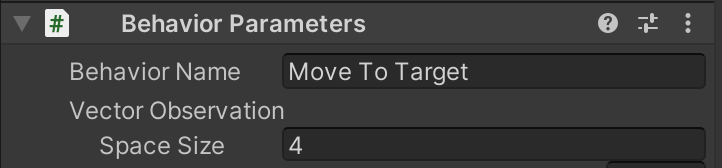
\includegraphics[width=0.9\textwidth]{space_size.png}
  \caption{Space Size}
\end{figure}

\vspace{1cm}

\newpage

\section{Beyin Oluşturma Kaydetme ve Yükleme}
\rule{\textwidth}{0.5pt}
\begin{enumerate}
\item  Unity projesi çalıştırıldığından itibaren Agentlar öğrenmeye başlar. Öğrenmiş olan bu beyin, proje dosyasının içindedir\\[5pt]

\begin{figure}[h]
  \centering
  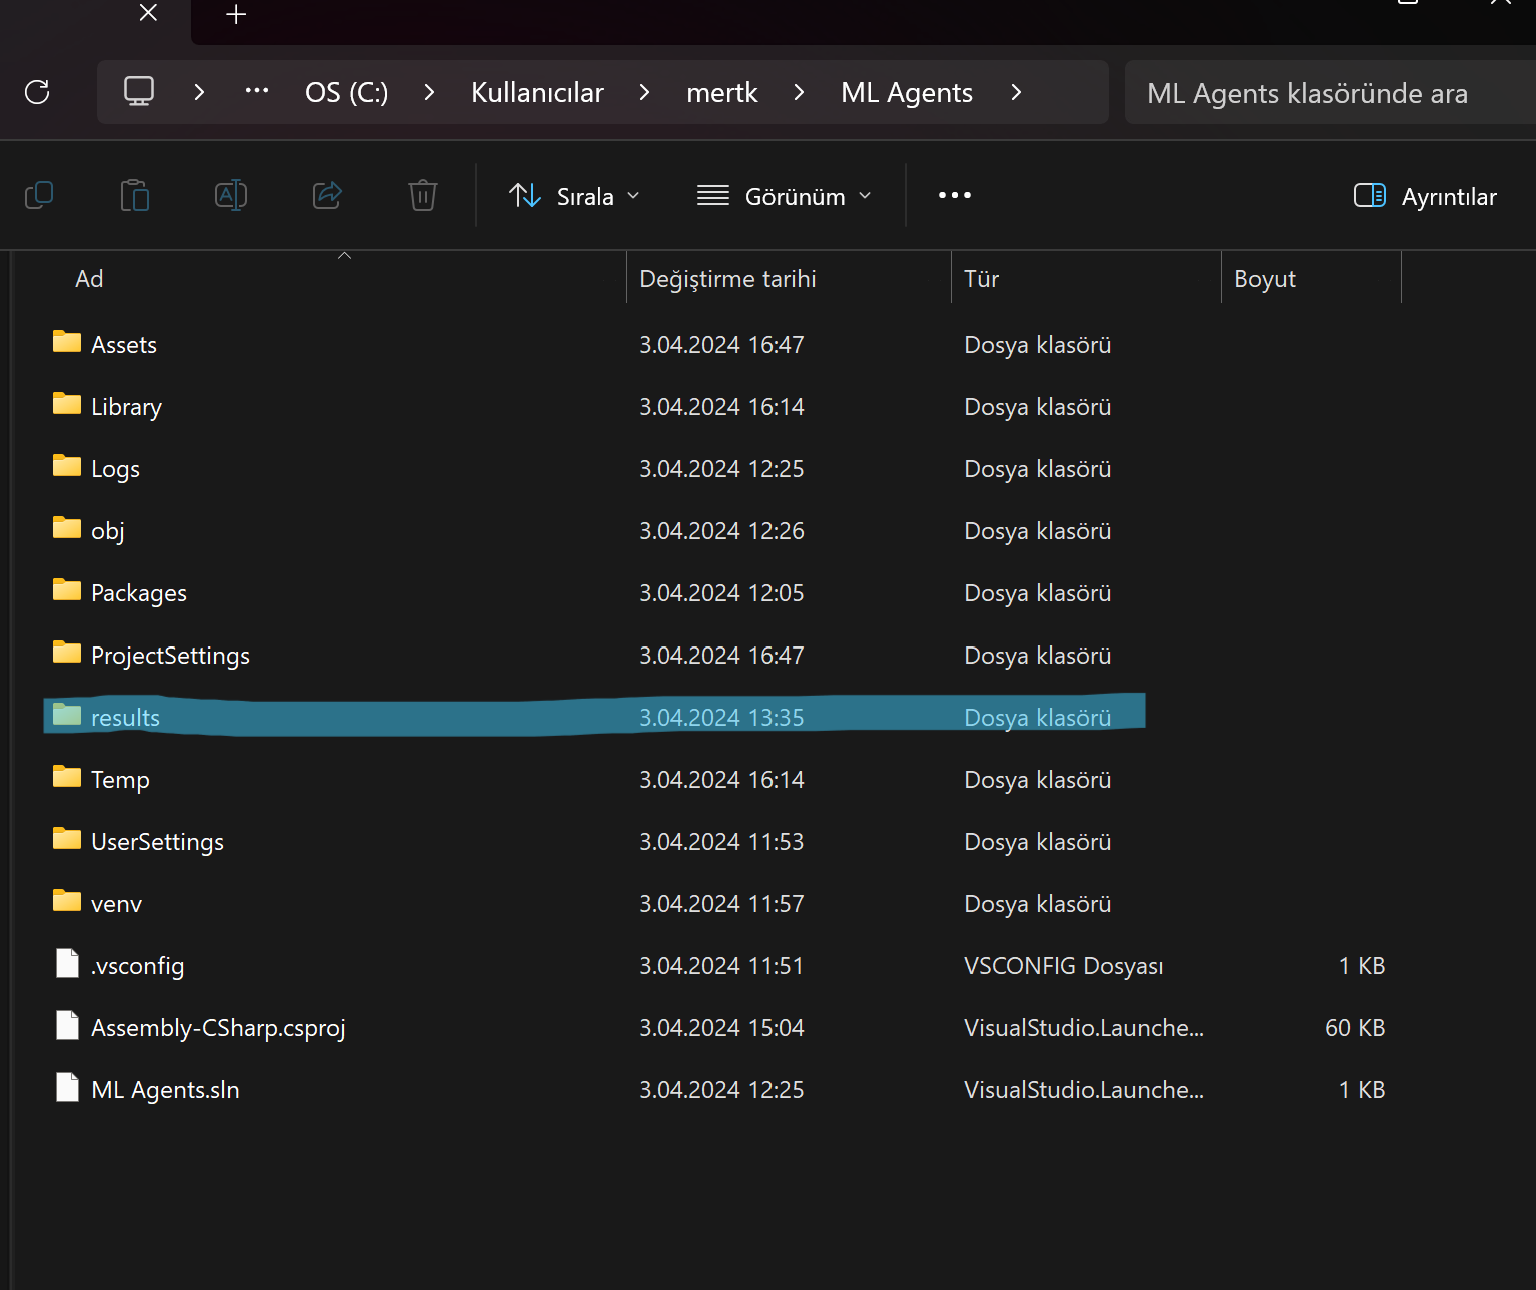
\includegraphics[width=1\textwidth]{results.png}
  \caption{Proje Dosyaları}
\end{figure}

\vspace{1cm}

\begin{figure}[h]
  \centering
  
\includegraphics[width=1\textwidth]{beyin.png}
  \caption{Beyin Dosyası}
\end{figure}

\newpage

\item Result dosyasının içindeki beyin, proje dosyasının içindeki Assets klasörüne kopyalanır. Kopyalanan bu beyin Unity içerisinde Assets kısmında görülebilir.

\begin{figure}[h]
  \centering
  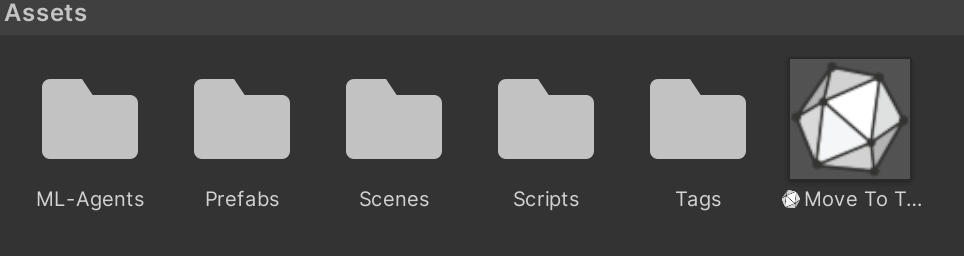
\includegraphics[width=1\textwidth]{assets_beyin.png}
  \caption{Assets Klasörü}
\end{figure}

\vspace{1cm}

\item Agent altında, Behavior Parameters bileşeninin içindeki, Model adındaki değişkene Assets klasöründeki beyin atanır. Böylece önceden eğitilen bir Agent'ı projeye eklemiş oluruz.

\begin{figure}[h]
  \centering
  
\includegraphics[width=1\textwidth]{brain_model.png}
  \caption{Model Değişkeni}
\end{figure}

\end{enumerate}

\newpage

\section{Başarılı ve Başarısız Oranı}
\rule{\textwidth}{0.5pt}

\par  Ekranın sol üst kısmında başarılı deneme sayısını, başarısız deneme sayısını, başarılı ve başarısız deneme sayısı arasındaki farkı ve başarı oranını gösteren bir panel yer almaktadır. Bu panel sayesinde deneme sayısı arttıkça başarı oranının arttığı gözlemlenebilir.\\[5pt]

\begin{figure}[h]
  \centering
  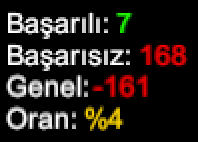
\includegraphics[width=0.7\textwidth]{basarisiz.png}
  \caption{Az Deneme Sayısı}
\end{figure}

\begin{figure}[h]
  \centering
  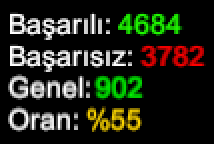
\includegraphics[width=0.7\textwidth]{basarili.png}
  \caption{Çok Deneme Sayısı}
\end{figure}

\newpage

\par Eğitim tamamlandıktan sonra TensorBoard yardımıyla sonuçlar grafik halinde görüntülenebilir. Aşağıdaki grafikler eğitilmiş bir beyine aittir.\\[5pt]

\begin{figure}[h]
  \centering
  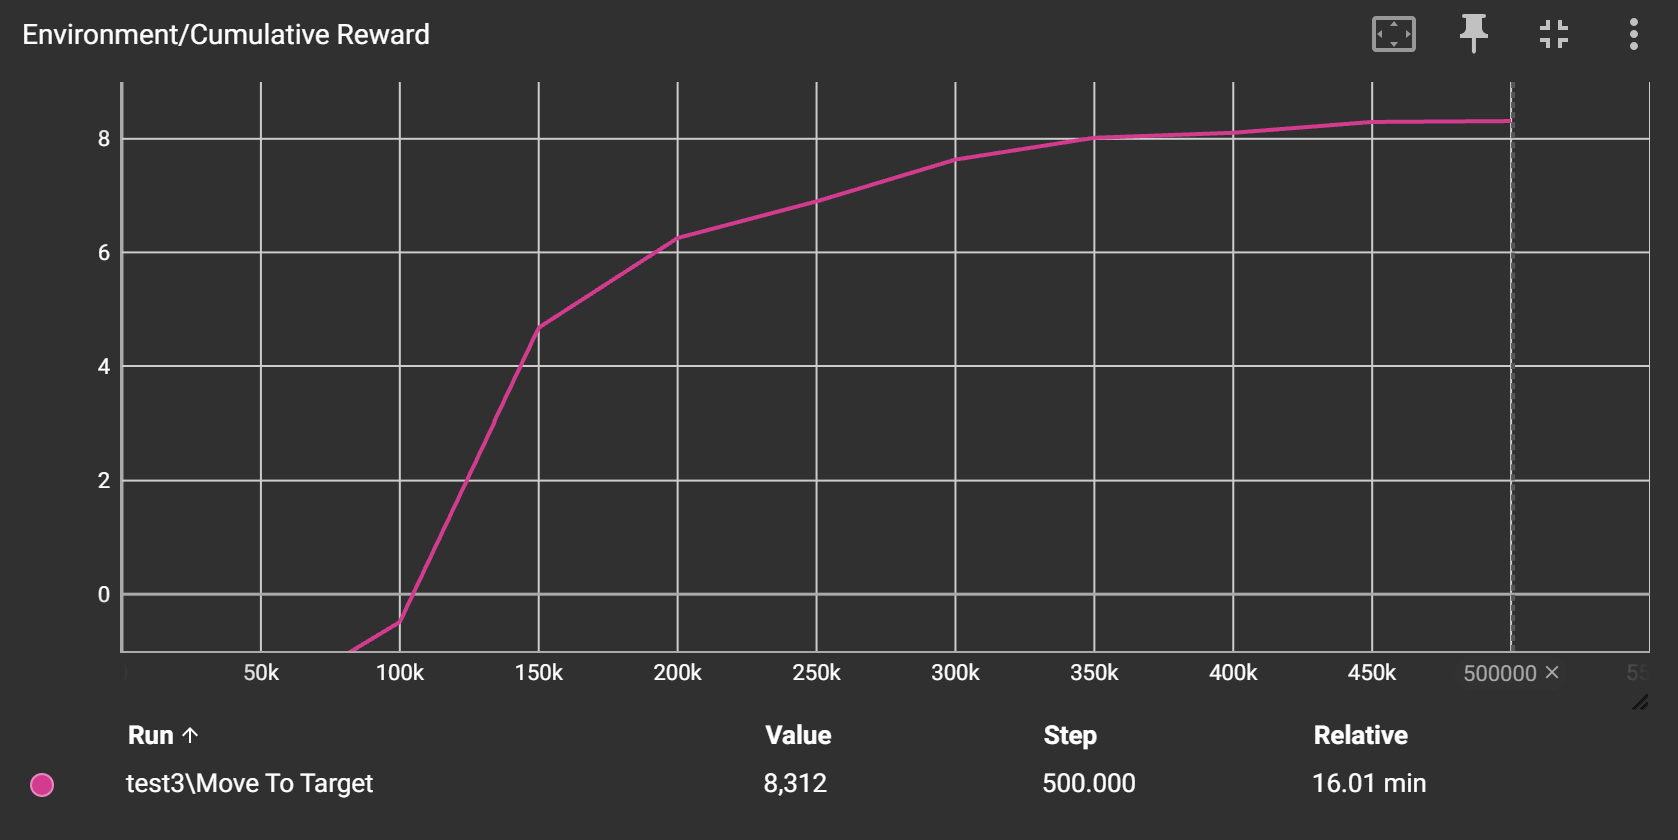
\includegraphics[width=0.9\textwidth]{reward-grap.png}
  \caption{Toplam Ödül Sayısı Grafiği}
\end{figure}

\begin{figure}[h]
  \centering
  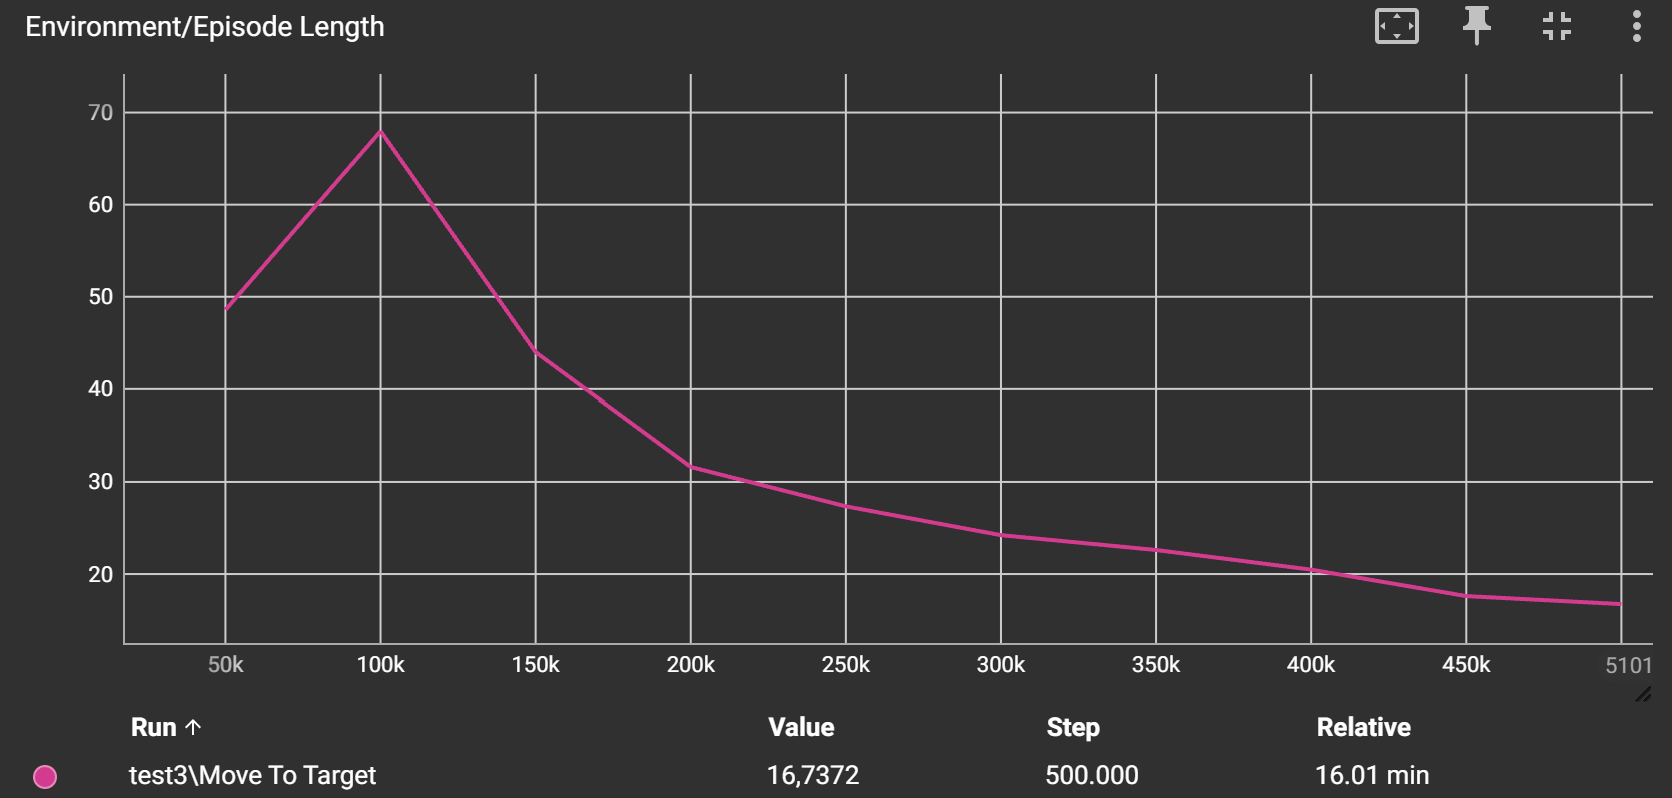
\includegraphics[width=0.9\textwidth]{episode-len.png}
  \caption{Bölüm Uzunluğu Grafiği}
\end{figure}

\newpage


\section{Viraj Dönmeyi Öğretme Projesi}
\rule{\textwidth}{0.5pt}
\par Ajanın sağa ve sola dönmeyi öğrenmesi için basit virajlardan oluşan bir bölüm tasarlandı ve çoğaltıldı. Önceki örneklere benzer şekilde ajan duvara temas ettiğinde negatif puan alıp baştan başlar. Kontrol noktasına temas ederse pozitif puan alır ve bir sonraki kontrol noktası belirir. Kontrol noktasının sırası arttıkça ajana vereceği ödül de artar.  \\[5pt]

\begin{figure}[h]
    \begin{center}
        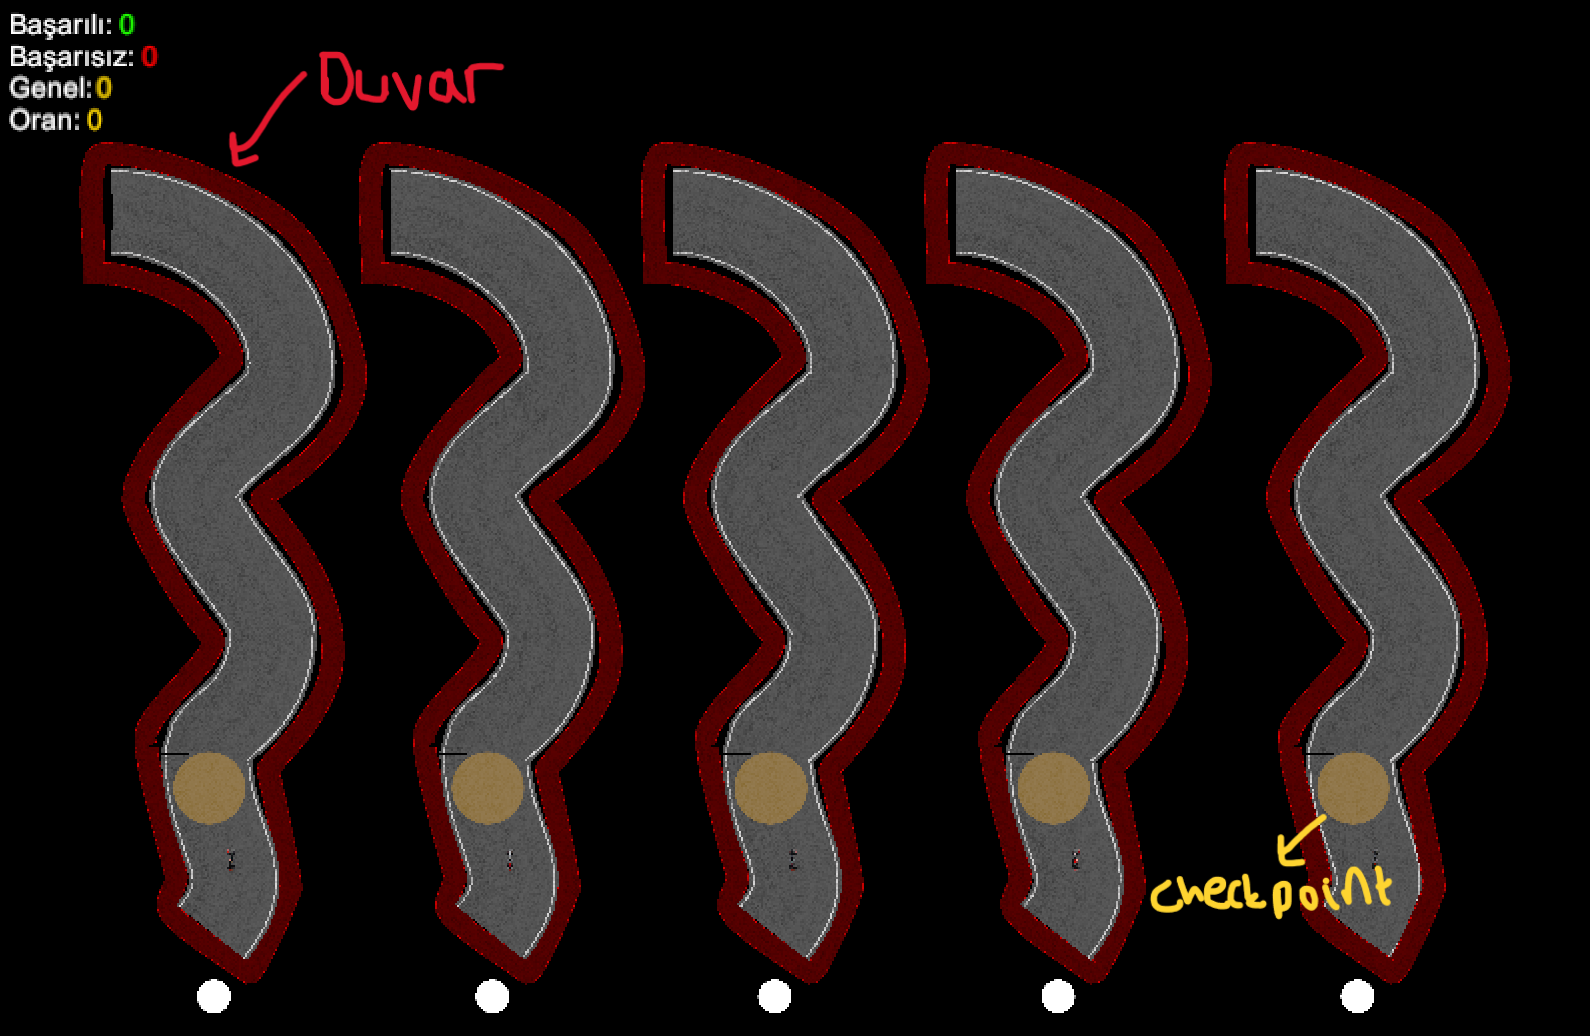
\includegraphics[width=1\textwidth]{5_pist.png}
    \end{center}
      \caption{Virajlı Bölüm Tasarımı \cite{sprite_shape}}
\end{figure}

\newpage

\subsection{Kontrol Noktaları}
\rule{\textwidth}{0.5pt}
\par Ajan, kontrol noktalarından birine temas ettiğinde bir sonraki kontrol noktasını aktive eder. Kontrol noktalarının verdiği ödül sırasına göre katlanarak artar. Son kontrol noktasına ulaşan ajan en baştan başlar. Eğer ajan bu esnada duvarla temas ederse en baştan başlar ve kontrol noktaları sıfırlanır. \\[5pt]

\begin{figure}[h]
    \begin{center}
        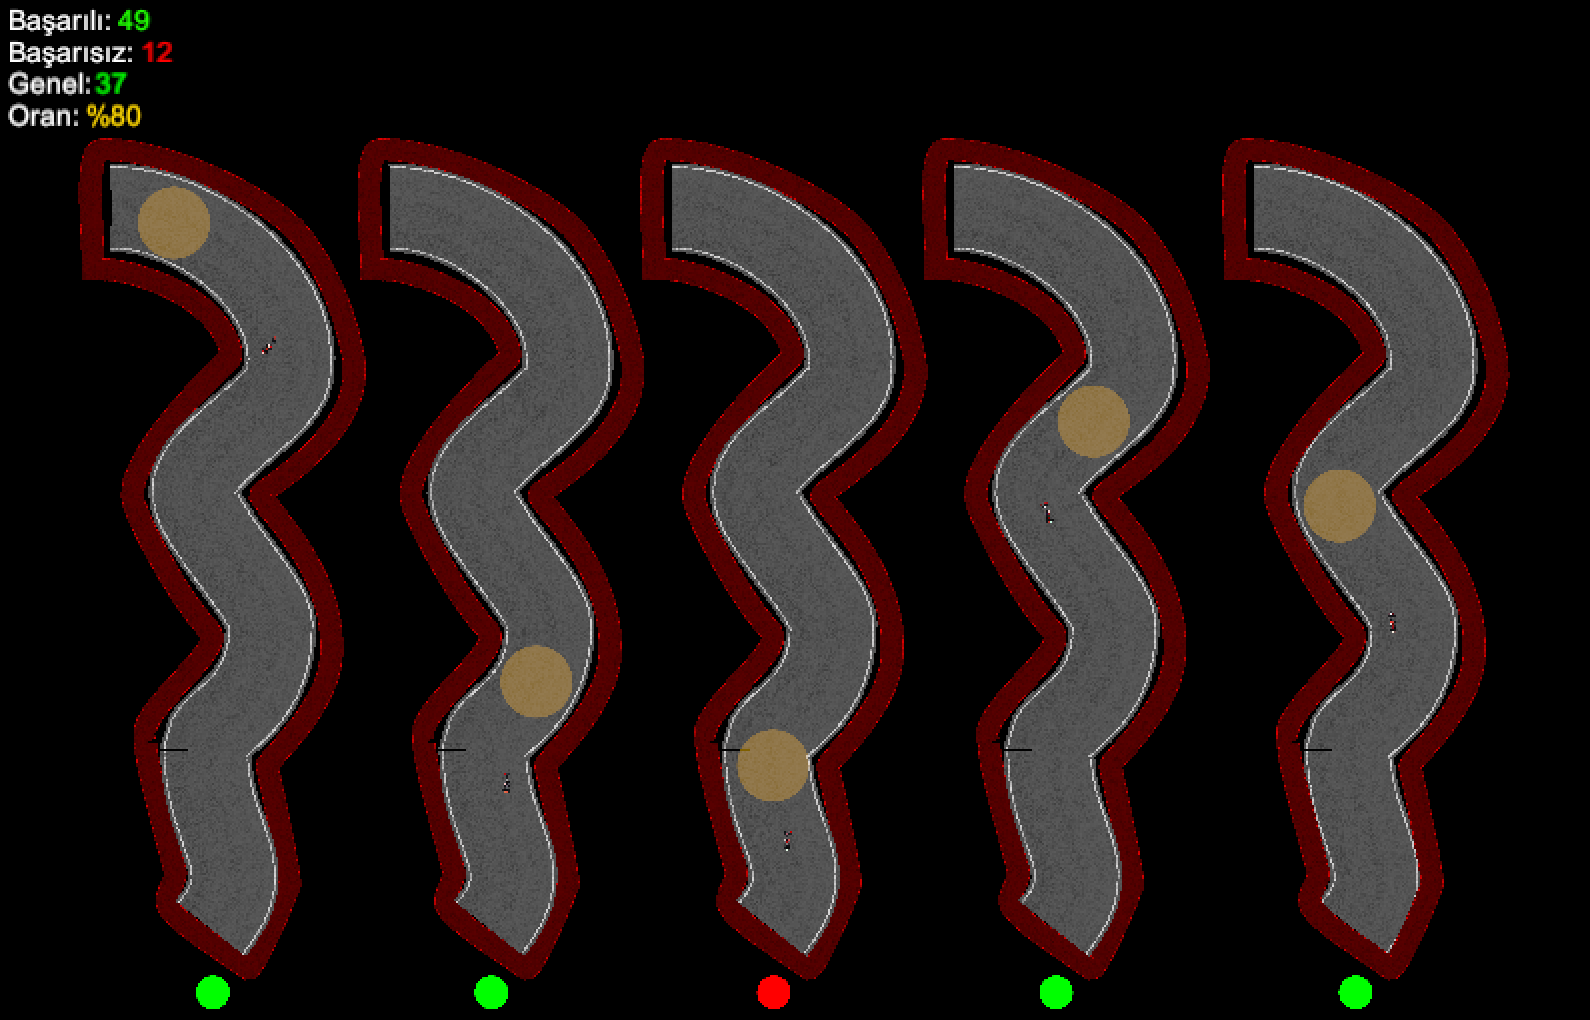
\includegraphics[width=1\textwidth]{checkpoint.png}
    \end{center}
      \caption{Sırayla Beliren Kontrol Noktaları}
\end{figure}

\newpage 

\section{Önceden Tasarlanmış Pistin Öğrenime Hazır Hale Getirilmesi}
\rule{\textwidth}{0.5pt}
\par Ajanın önceden tasarlanan pist etrafında tur atabilmesi için piste oldukça sık şekilde kontrol noktaları yerleştirildi. Bu sayede ajan, bir kontrol noktasına ulaştığında, bir sonraki kontrol noktasına ulaşması için gereken çaba miktarı azaltıldı. \\[5pt]

\begin{figure}[h]
    \begin{center}
        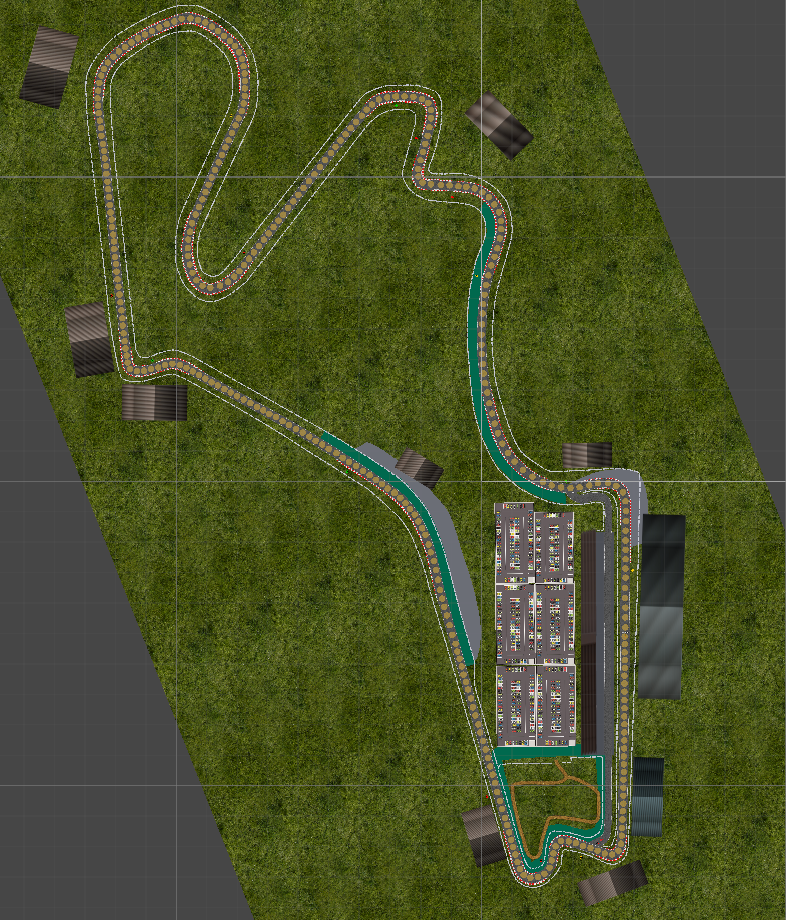
\includegraphics[width=0.9\textwidth]{cp_big.png}
    \end{center}
      \caption{Pist}
\end{figure}

\newpage

\subsection{Pist Üzerindeki Kontrol Noktaları}
\rule{\textwidth}{0.5pt}
\par Ajan, ilk kontrol noktasına temas ettiğinde, temas ettiği kontrol noktası bir sonraki kontol noktasına taşınır. İlk başta birinci kontrol noktası dışında aktif olmayan diğer kontrol noktaları, birinci kontrol noktasının önceden belirlenmiş pozisyona taşınması için kullanılır\cite{CP}.  \\[5pt]

\begin{figure}[h]
    \begin{center}
        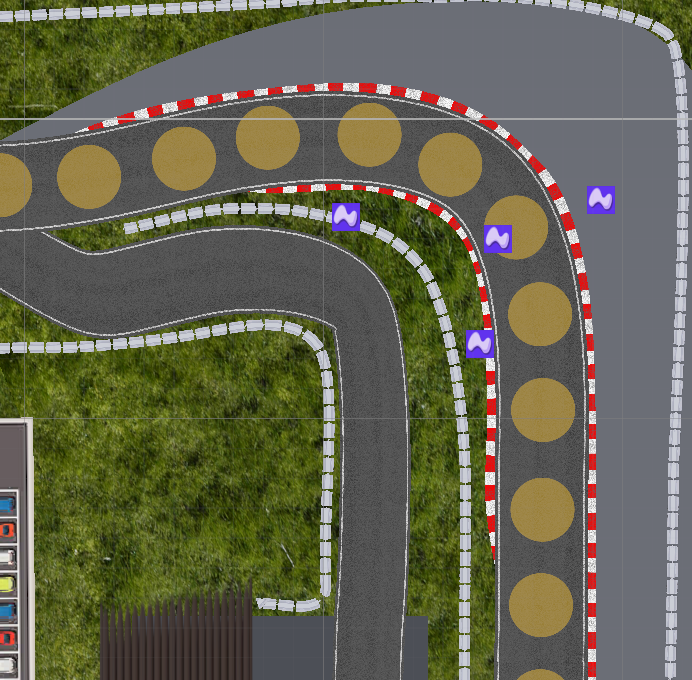
\includegraphics[width=1\textwidth]{cp_small.png}
    \end{center}
      \caption{Pist Üzerindeki Kontrol Noktaları}
\end{figure}

\newpage

\section{Ray Perception Sensor 2D}
\rule{\textwidth}{0.5pt}
\par Kullanıldığı objenin etrafındaki nesneleri algılamak için kullanılır\cite{Ray}. Projede ajan üzerinde kullanılan bu sensör, kontrol noktalarını ve duvarları algılamak için kullanılır. \\[5pt]

\begin{figure}[h]
    \begin{center}
        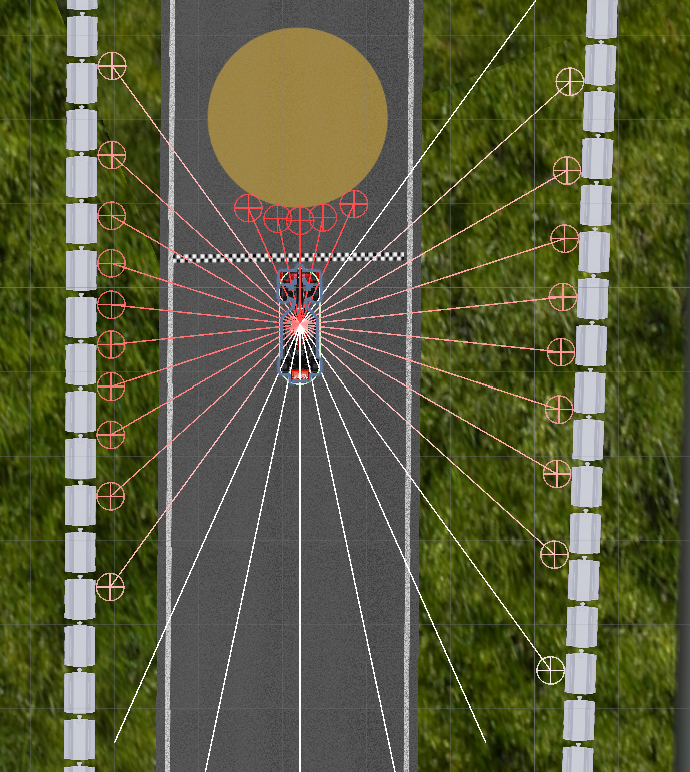
\includegraphics[width=1\textwidth]{ray.png}
    \end{center}
      \caption{Ray Perception Sensor}
\end{figure}

\newpage

\section{Taklit Öğrenmesi (Imitation Learning)}
\rule{\textwidth}{0.5pt}
\par Taklit öğrenmesi ajanın, önceden kullanıcı tarafından kaydedilen davranışları taklit ederek yeni davranışlar sergilemesini sağlayan algoritmadır. Ajanın, hedefin hangi yönde olduğunu anlaması için gerekli gözlemler eklendi. \\[5pt]

\subsection{Oluşturulan Dosyalar}
\par Taklit öğrenme algoritmasını kullanmak için proje dosyasında "config" ve "Demos" adlı iki klasör oluşturulmalıdır\cite{imitation2}. \\[5pt]

\subsubsection{Config Klasörü}
\par Config Dosyasının içine MoveToTarget isimli .yaml uzantılı bir text dosyası oluşturuldu. Bu text dosyası ajanın eğitilmesi için gerekli olan parametreleri değiştirilmesine olanak sağlar. Kaydedilen demo dosyasının konumu bu dosya içinde belirtilmelidir.\cite{imitation1}. \\[5pt]

\subsubsection{Demos Klasörü}
\par Demos klasörü kullanıcı tarafından kaydedilen davranışların kaydedildiği klasördür. .demo uzantısına sahiptir. \\[5pt]

\subsubsection{Ajanın Hedefe Göre Yönü}
\par Ajanın gözlem topladığı kod kısmına, ajanın hedefe göre yön vektörünü alan bir gözlem eklendi\cite{dir}. \\[5pt]

\newpage

\section{Davranışların Kaydedilmesi}
\rule{\textwidth}{0.5pt}
\par Kullanıcı davranışlarını kaydetmek için, bir ML-Agents bileşeni olan Demonstration Recorder kullanılır. Kayıtı başlatmak için Record yazısının yanındaki kutucuk işaretlenmelidir. \\[5pt]

\begin{figure}[h]
    \begin{center}
        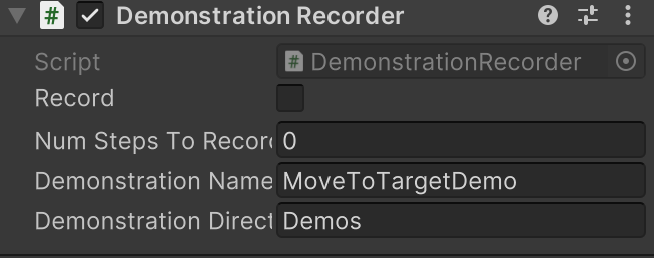
\includegraphics[width=0.8\textwidth]{demo.png}
    \end{center}
      \caption{Demonstration Recorder}
\end{figure}

\vspace{5pt}

\section{Eğitimler}
\rule{\textwidth}{0.5pt}
\par Doğru parametreler, doğru ödül, ceza miktarları girildikten sonra ajan hareket etmeye başlar. Başlarda çember şeklinde hareket eden ajan eğitim devam ettikçe düz gitmeyi, sonrasında virajları dönmeyi öğrenir. 33 turluk bir eğitim sürecinde 3 dakika 55 saniye 665 saliselik en iyi tur zamanı elde edilmiştir. \\[5pt]
\begin{figure}[h]
    \begin{center}
        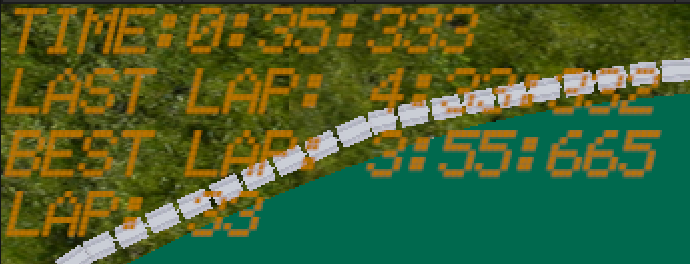
\includegraphics[width=0.8\textwidth]{best_time.png}
    \end{center}
      \caption{En İyi Tur Zamanı}
\end{figure}

\newpage

\subsection{Eğitim-1}
\rule{\textwidth}{0.5pt}
\par Önceki çalışmadaki ödül ve ceza sistemini değiştirmeden yapılan eğitimde ajan, direksiyon hareketleri ve geri gitmesi için ceza almaktadır. Bu eğitim sonucu elde edilen veriler aşağıdaki gibidir.\\[5pt]

\begin{figure}[h]
    \begin{center}
        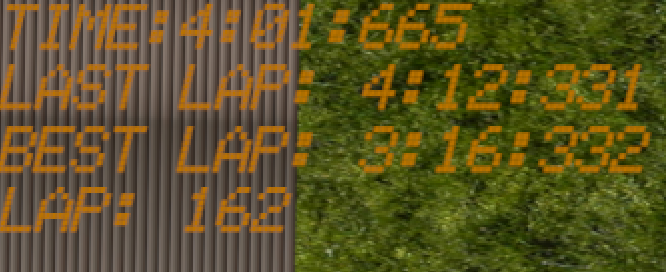
\includegraphics[width=1\textwidth]{egitim.png}
    \end{center}
      \caption{Eğitim-1}
\end{figure}

\subsection{Eğitim-2}
\rule{\textwidth}{0.5pt}
\par Önceki çalışmadan farklı olarak ajanın direksiyon hareketlerine ve geri gitmesine ceza verilmeyen sistemde alınan sonuçlar aşağıdaki gibidir.

\begin{figure}[h]
    \begin{center}
        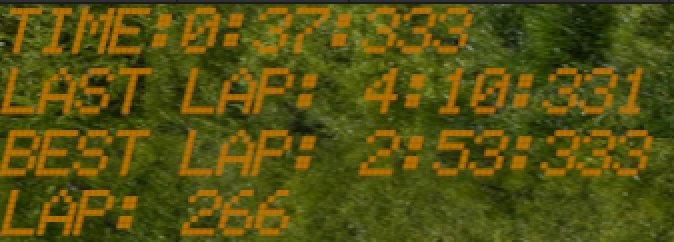
\includegraphics[width=1\textwidth]{egitim2.png}
    \end{center}
      \caption{Eğitim-2}
\end{figure}


\subsection{Eğitim-3}
\rule{\textwidth}{0.5pt}
\par Ödül ve ceza sistemi değiştirilmeden, pist dışına çıkınca ajanın hızının ve yol tutuşunun azaltıldığı eğitimde alınan sonuçlar aşağıdaki gibidir.\\[5pt]

\begin{figure}[h]
    \begin{center}
        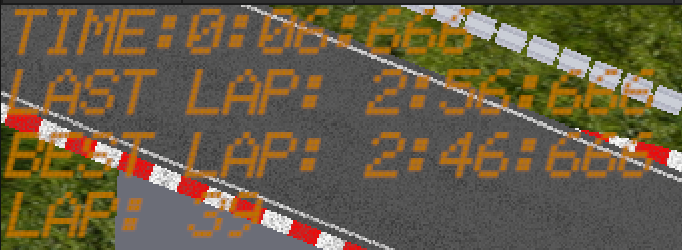
\includegraphics[width=1\textwidth]{egitim3.png}
    \end{center}
      \caption{Eğitim-3}
\end{figure}

\vspace{1cm}

\captionsetup[table]{justification=raggedright, singlelinecheck=false}


\renewcommand{\tablename}{Tablo}
\begin{table}[h!]
\centering
  \Large % Yazı boyutunu artırmak için
    \caption {Yöntemler ve Zamanlar}
  \begin{tabular}{|c|c|c|}
    \hline
    Eğitim & Yöntem & Zaman \\
    \hline
    1 & Eski Ödül Ceza Sistemi & 3:16:332 \\
    \hline
    2 & Yeni Ödül Ceza Sistemi & 2:53:333 \\
    \hline
    3 & Hız ve Yol Tutuşu Ayarlamaları & 2:46:666 \\
    \hline
  \end{tabular}
\end{table}

\newpage

\section{Denemeler}
\rule{\textwidth}{0.5pt}
\par Önceki eğitimlerdeki gözlemler ışığında yapılan denemeler aşağıda gösterilmiştir.\\[5pt]

\subsection{Deneme-1}
\rule{\textwidth}{0.5pt}
\par Önceki çalışmadaki ödül ve ceza sistemini değiştirmeden, ajanın sık sık hata yaptığı virajlara ceza puanı veren bölgeler yapılmıştır. Önceki çalışmalara göre bir gelişme gözlemlenmemiştir.\\[5pt]

\begin{figure}[h]
    \begin{center}
        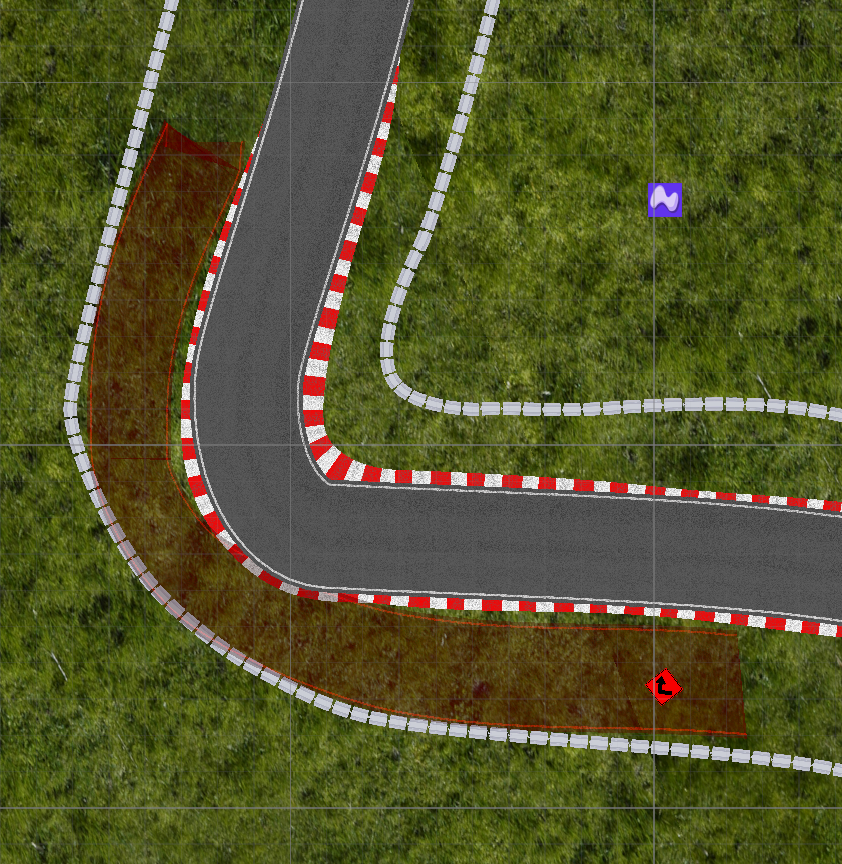
\includegraphics[width=0.9\textwidth]{penalty.png}
    \end{center}
      \caption{Hata Yapılan Virajdaki Ceza Bölgesi}
\end{figure}

\newpage

\subsection{Deneme-2}
\rule{\textwidth}{0.5pt}
\par Önceki çalışmadaki ödül ve ceza sistemini değiştirmeden, kontrol noktalarının içine daha küçük kontrol noktaları eklenerek ajanın pisti daha doğru şekilde takip etmesi amaçlanmıştır. Önceki çalışmalara göre bir gelişme gözlemlenmemiştir.

\begin{figure}[h]
    \begin{center}
        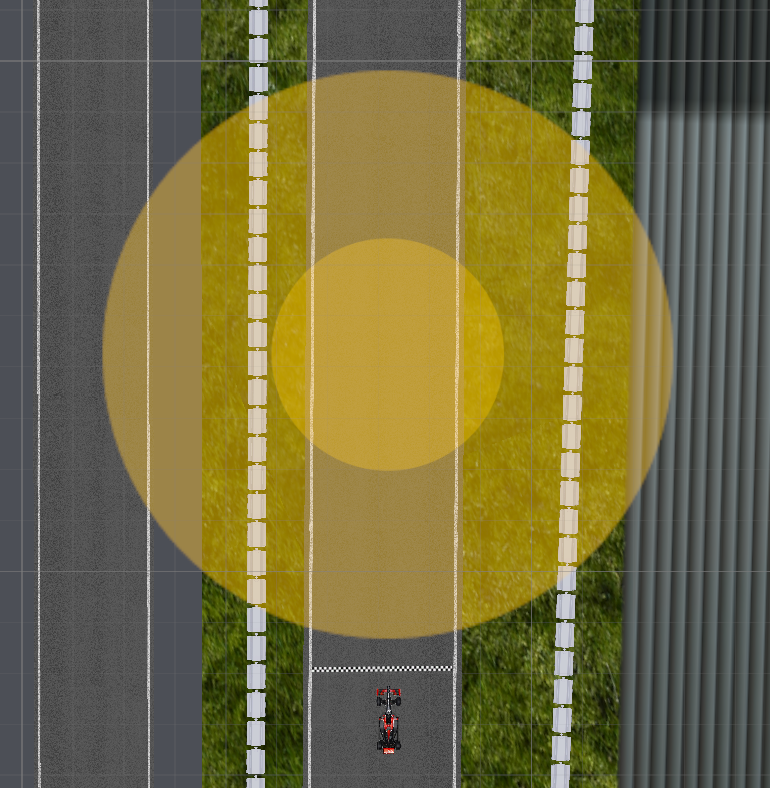
\includegraphics[width=0.8\textwidth]{cp.png}
    \end{center}
      \caption{Küçük Kontrol Noktası}
\end{figure}

\vspace{1cm}

\subsection{Deneme-3}
\rule{\textwidth}{0.5pt}
\par Yukarıda bahsedilen deneme-1 ve deneme-2 yöntemlerini birleştirerek yapılan denemede önceki çalışmalara göre bir gelişme gözlemlenmemiştir.\\[5pt]

\subsection{Deneme-4}
\rule{\textwidth}{0.5pt}
\par Deneme-1, deneme-2 ve deneme-3 tarafından kullanılan yöntemler sonucunda bir gelişme gözlemlenmediği için geçmiş çalışmadaki sisteme geri dönülmüştür. Farklı olarak, ajan 20 saniye içinde hedefe ulaşamazsa bir önceki kontrol noktasına geri dönmesi yerine artık ajan herhangi bir duvara çarptığında önceki kontrol noktasına geri döner. Bu ve önceki denemeler sonucu alınan süreler aşağıdaki gibidir.\\[5pt]

\begin{figure}[h]
    \begin{center}
        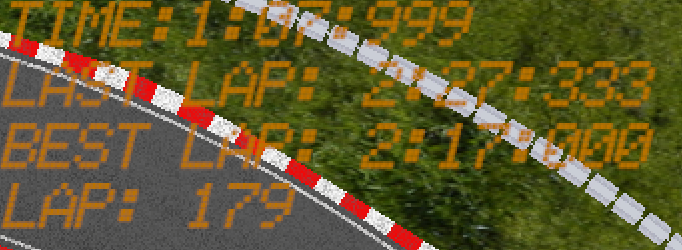
\includegraphics[width=1\textwidth]{time.png}
    \end{center}
      \caption{Son Çalışmadaki En İyi Zaman}
\end{figure}

\vspace{1.5cm}

\captionsetup[table]{justification=raggedright, singlelinecheck=false}

\renewcommand{\tablename}{Tablo}
\begin{table}[h!]
\centering
  \Large % Yazı boyutunu artırmak için
    \caption {Çalışmalar ve Zamanlar}
  \begin{tabular}{|c|c|c|}
    \hline
    Hafta & Yöntem & Zaman \\
    \hline
    10 & Duvar \& Kontol Noktası Ayarlamaları & 2:17:000 \\
    \hline
    9 & Hız \& Yol Tutuşu Ayarlamaları & 2:46:666 \\
    \hline
    8 & İlk Eğitim & 3:55:665 \\
    \hline
  \end{tabular}
\end{table}

\newpage

\thispagestyle{empty}
\begin{landscape}

\raisebox{5cm}[0pt][0pt]

\captionsetup[table]{justification=raggedright, singlelinecheck=false}

\renewcommand{\tablename}{Tablo}
\renewcommand{\arraystretch}{1.5} % Satır yüksekliğini artırmak için

\begin{table}[h!]
\centering
  \Large % Yazı boyutunu artırmak için
    \caption {Ödüller ve Cezalar}
  \begin{tabular}{|c|c|c|}
    \hline
    \textbf{Davranış} & \textbf{Ödül Artış Miktarı} & \textbf{Etken}\\
    \hline
    Kontrol Noktasına Ulaşma & +100 & Yok \\
    \hline
    Duvara Çarpma & -3500 & Yok \\
    \hline
    20 Saniye İçinde Kontrol Noktasına Ulaşamazsa & -1000 & Her Seferinde 2 Katı \\
    \hline
    Kontrol Noktasına Yaklaşıyorsa & +1 & Her Frame Başı \\
    \hline
    Kontrol Noktasından Uzaklaşıyorsa & -3 & Her Frame Başı \\
    \hline
    Kontrol Noktasının Ajana Uzaklığı & +5 / Uzaklık & Her Frame Başı \\
    \hline
    Hedefe Ulaşamadığı Süre Boyunca & -1 & Her Frame Başı \\
    \hline
  \end{tabular}
\end{table}

\end{landscape}

\newpage

\section{Ajan Girdileri}
\rule{\textwidth}{0.5pt}
\par Ajanın hangi girdileri gönderdiğini görsel olarak görebilmek için ekranın sağ üst köşesine ekleme yapıldı.\\[5pt]

\begin{figure}[h]
    \begin{center}
        
\includegraphics[width=1\textwidth]{wasd.png}
    \end{center}
      \caption{Ajan Girdileri}
\end{figure}

\newpage

\section{Sonuç}
\rule{\textwidth}{0.5pt}
 \par ML-Agents kullanılarak Unity içinde yapay zeka eğitimi yapılabilmektedir. Bu proje kapsamında, ajanların araç kontrolünü öğrenmesi hedeflenmiştir. Bunun için ML-Agents kütüphanesi kullanılmış ve çeşitli eğitimler yapılmıştır. Eğitim sonuçlarına bakıldığında, ajanların belirli bir hedefe doğru hareket etme yeteneğinin geliştirildiği görülmektedir.\\[5pt]

\par Kullanılan teknolojiler, Unity oyun motoru, ML-Agents kütüphanesi, Python programlama dili ve PyTorch kütüphanesidir. Bu teknolojilerin bir araya getirilmesiyle yapay zeka eğitimi için etkili bir platform oluşturulmuştur.\\[5pt]

\par Proje, önceden tasarlanmış bir pist etrafında araç kontrolünü öğrenmek için çeşitli senaryoları içermektedir. Ajanların başarılı bir şekilde bu senaryoları tamamlaması, ML-Agents'in etkinliğini ve kullanışlılığını göstermektedir.\\[5pt]

\par Son olarak, proje ML-Agents ve Unity'nin yapay zeka eğitimi alanındaki potansiyelini ortaya koymaktadır.\\[5pt]
\par 

\newpage

\bibliographystyle{ieeetr}
\bibliography{ref}

\end{document}
